\section{Results}
\label{sec:results}

\subsection{AIMSpice}

The register could have different effect and operations due to the corner of the transistor and the temperature. There are five corners the transistors could be; TT(typical-typical), SS(slow-slow), FF(fast-fast), SF(slow-fast) and FS(fast-slow).  For all of the corners they have been tested for three temperatures, 0$^\circ C$, 27$^\circ C$ and 70$^\circ C$. All the different plots for the different cases are shown in the \autoref{appendix:register_plots}. 

To validate the functionality of the register, one can examine the plot of the TT corner at 27$^\circ C$. 

\begin{figure}[H]
    \centering
    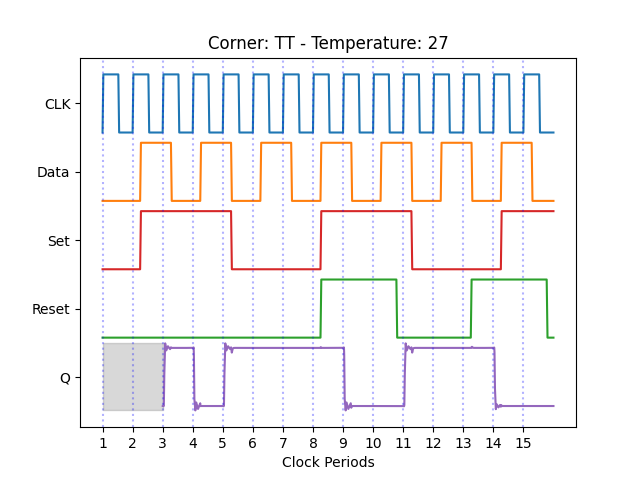
\includegraphics[width=0.9\textwidth]{Figures/Aimspice_Plots/TT_27.png}
    \caption{Plot of register for TT corner}
    \label{fig:result_TT27}
\end{figure}

We have also looked at the stability of the register, when changing from low to high, and how they different corners or temperatures affect it. \autoref{fig:TT_diffTemps} and \autoref{fig:27_diffCorners} shows the stability for the same corner with different temperatures and different corners at same temperature respectively. The other plots for the different corners and temperatures can be found in \autoref{appendix:register_stability}.

\begin{figure}[H]
    \begin{minipage}{0.5\textwidth}
        \centering
        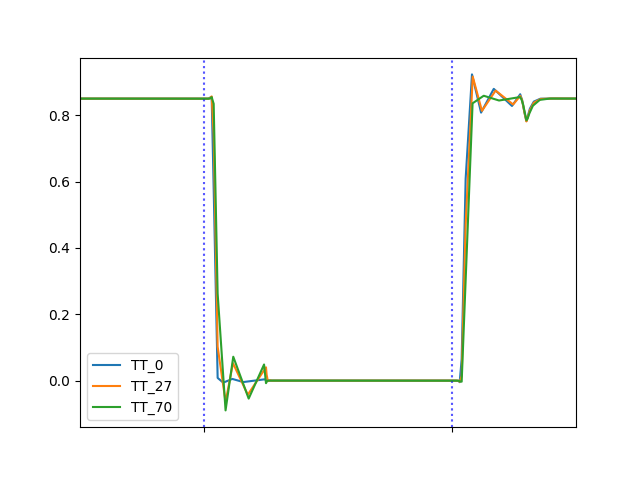
\includegraphics[width=\textwidth]{Figures/Aimspice_Plots/CornerTT.png}
        \caption{\parbox{0.5\textwidth}{Plot of TT corner at different temperatures.}}
        \label{fig:TT_diffTemps}
    \end{minipage}%
    \begin{minipage}{0.5\textwidth}
        \centering
        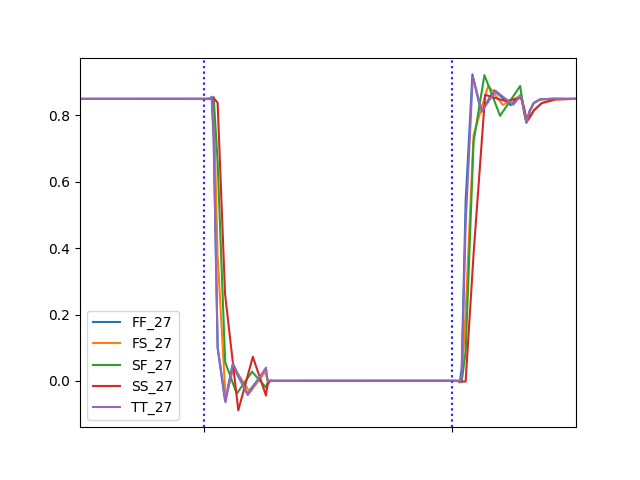
\includegraphics[width=\textwidth]{Figures/Aimspice_Plots/Temperatur27.png}
        \caption{\parbox{0.4\textwidth}{Plot of the different corners at 27 $^\circ$C}}
        \label{fig:27_diffCorners}
    \end{minipage}
\end{figure}

\subsubsection{Static Power Consumption}

As explained in section \ref{subsec:low_power}, a low voltage on $V_{DD}$ is optimal. We have therefore chosen a value for $V_{DD} = 0.85V$, as a lower $V_{DD}$ gives a lower power consumption. By using the function operating point in AIMSpice, the leakage current in the $V_{DD}$ node can be found.

Table \ref{tab:leakage} shows the different leakage current for the TT and FF corners with all three temperatures. To calculate the static power consumption, we use the formula \ref{eq:power} for all the values and get table \ref{tab:power}.

\begin{table}[H]
\centering
\caption{Leakage Current}
\label{tab:leakage}
\resizebox{0.4\columnwidth}{!}{%
    \begin{tabular}{lll}
    \cline{2-3}
    \multicolumn{1}{l|}{} &
      \multicolumn{1}{l|}{\cellcolor[HTML]{C0C0C0}TT} &
      \multicolumn{1}{l|}{\cellcolor[HTML]{C0C0C0}FF} \\ \hline
    \multicolumn{1}{|l|}{\cellcolor[HTML]{C0C0C0}0 $^\circ$C} &
      \multicolumn{1}{l|}{1.0931 nA} &
      \multicolumn{1}{l|}{3.1854 nA} \\ \hline
    \multicolumn{1}{|l|}{\cellcolor[HTML]{C0C0C0}27 $^\circ$C} &
      \multicolumn{1}{l|}{3.0325 nA} &
      \multicolumn{1}{l|}{8.5711 nA} \\ \hline
    \multicolumn{1}{|l|}{\cellcolor[HTML]{C0C0C0}70 $^\circ$C} &
      \multicolumn{1}{l|}{6.9843 nA} &
      \multicolumn{1}{l|}{13.513 nA} \\ \hline
     &  &  
    \end{tabular}%
}
\end{table}

\begin{table}[H]
\centering
\caption{Static Power Consumption}
\label{tab:power}
\resizebox{0.4\columnwidth}{!}{%
\begin{tabular}{lll}
\cline{2-3}
\multicolumn{1}{l|}{} &
  \multicolumn{1}{l|}{\cellcolor[HTML]{C0C0C0}TT} &
  \multicolumn{1}{l|}{\cellcolor[HTML]{C0C0C0}FF} \\ \hline
\multicolumn{1}{|l|}{\cellcolor[HTML]{C0C0C0}0 $^\circ$C} &
  \multicolumn{1}{l|}{0.92914 nW} &
  \multicolumn{1}{l|}{2.7076 nW} \\ \hline
\multicolumn{1}{|l|}{\cellcolor[HTML]{C0C0C0}27 $^\circ$C} &
  \multicolumn{1}{l|}{2.5776 nW} &
  \multicolumn{1}{l|}{7.2854 nW} \\ \hline
\multicolumn{1}{|l|}{\cellcolor[HTML]{C0C0C0}70 $^\circ$C} &
  \multicolumn{1}{l|}{5.9367 nW} &
  \multicolumn{1}{l|}{11.486 nW} \\ \hline
 &  &  
\end{tabular}
}
\end{table}

\subsection{Verilog Testbenches}

In this subsection results of Verilog-simulations will be presented. All Verilog-code is given in \autoref{appendix:Verilog-code} and \ref{sec:verilog_testbenches}.

\subsubsection{FSM Results}
\label{subsubsec:fsm_results}

\noindent
The timing diagram generated by the FSM testbench is shown in \autoref{fig:fsm_simulation}. The timing diagram includes the input signals CLK and I[1:0], the output signal CTRL[1:0] (shown as O[1:0] in the figure) and the current state C[1:0], which is only an internal value in the FSM. For simplicity, values for I[1:0] and O[1:0] are shown in binary notation and C[1:0] in decimal notation.

\begin{figure}[H]
    \centering
    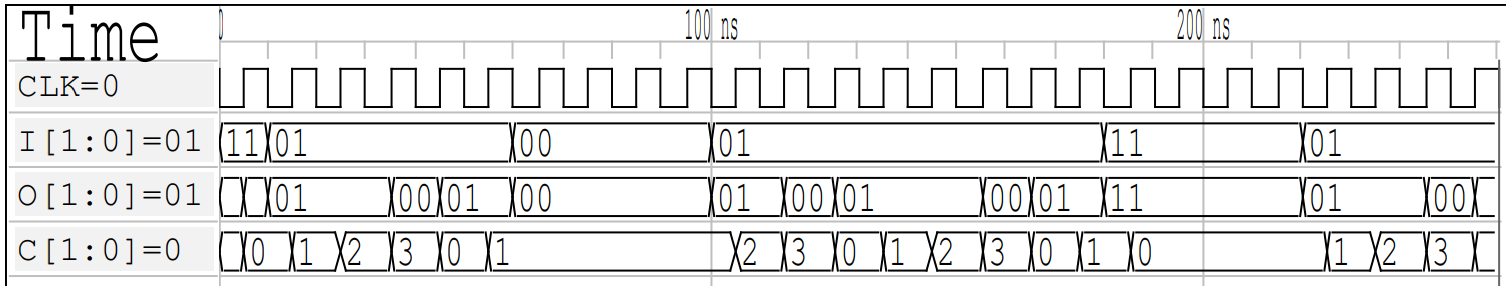
\includegraphics[width=\textwidth]{Figures/FSM_testbench_out.png}
    \caption{Timing diagram of FSM simulated in Verilog}
    \label{fig:fsm_simulation}
\end{figure}

The diagram shows the state register being reset on the first rising edge of the CLK. As the input changes to ''01'', the FSM cycles through the states 0, 1, 2, and 3. The first three states, 0, 1, and 2, output the control signals ''01'' meaning ''run a mac operation'', while state 3 outputs ''00'', meaning ''pause the MAC and hold the stored value''. When the input is ''00'', the FSM pauses on its current state before continuing when the input returns to ''01''. When the input is ''11'', the state is forced to ''00'' and the output is ''11'' which should reset the accumulator in the MAC.

\subsubsection{MAC Results}
\label{subsubsec:mac_results}

The output provided by the multiplier testbench is 

\begin{figure}[H]
\centering
\caption{Loop to check all combinations for the adder.}
\label{fig:verilog_adderTB_excerpt}
\begin{minipage}{0.8\textwidth}
\begin{lstlisting}[style=verilogStyle]
[Running] Multiplier_Testbench.v
VCD info: dumpfile Multiplier_Testbench.vcd opened for output.
0*0= 0
[...]
3*3= 9
No errors found
Multiplier_Testbench.v:34: $finish called at 16000 (1ps)
[Done] exit with code=0 in 0.522 seconds
\end{lstlisting}
\end{minipage}
\end{figure}






From the figure we see that the memory transitions to the expected states based on the inputs. The FSM begins in state ''Run-1'' and transitions to state ''Reset'' as the reset input $I_1$ is set high. The next state is ''Run-1'', then ''Run-2''. The Run-bit $I_0$ is then set low, resulting in a two-period pause in state ''Pause-2''. Further the FSM transitions to ''Run-3'', ''Pause'' and ''Run-1''.

This simulation was run and verified to follow the wanted behaviour as given by table x.

\autoref{fig:eightbitadder_sim} shows a simulation of the 8-bit adder with random 8-bit inputs A and B. Note that all values in the timing diagram are hexadecimal and that any overflow-bits are handled outside our system. The code used for this simulation is given in \autoref{verilog_eightbitadder}.

\begin{figure}[H]
    \centering
    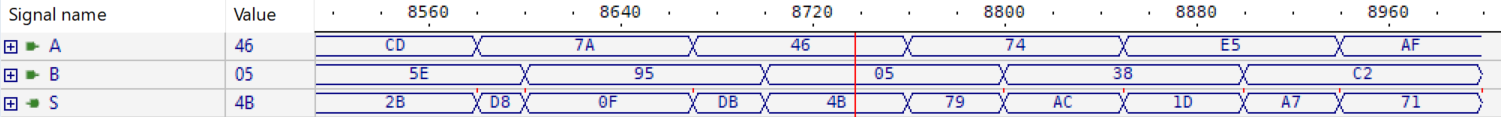
\includegraphics[width=\textwidth]{Figures/Test of eightbitadder.png}
    \caption{Timing diagram of 8-bit adder simulated in Verilog}
    \label{fig:eightbitadder_sim}
\end{figure}

\autoref{fig:dflipflop_sim} shows a simulation of a single D Flip-Flop realized in Verilog.

\begin{figure}[H]
    \centering
    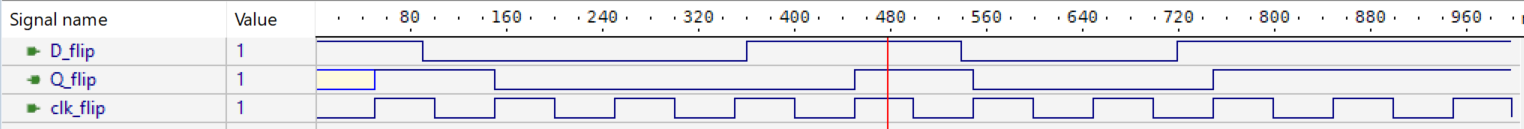
\includegraphics[width=\textwidth]{Figures/Test of Dflipflop.png}
    \caption{Timing diagram of D Flip-Flop simulated in Verilog}
    \label{fig:dflipflop_sim}
\end{figure}

\autoref{fig:8bitregister_sim} shows a simulation of a 8-bit register realized in Verilog.

\begin{figure}[H]
    \centering
    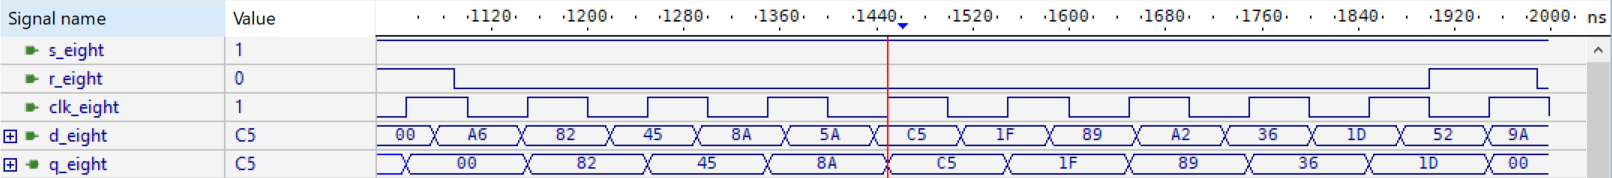
\includegraphics[width=\textwidth]{Figures/VerilogPlot_8bitreg.png}
    \caption{Timing diagram of an 8-bit register simulated in Verilog}
    \label{fig:8bitregister_sim}
\end{figure}

\autoref{fig:multiplier_sim} shows a simulation of the 2-bit multiplier realized in Verilog. Inputs A and B are stimulated with arbitrary two bit values to observe the possible outputs. The multiplier has a 4-bit output as the largest possible output result, 9, needs four bits to be represented in binary.

\begin{figure}[H]
    \centering
    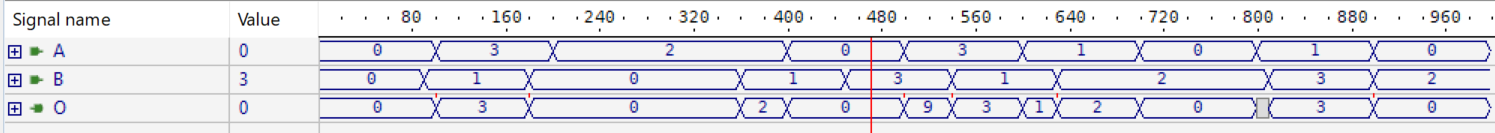
\includegraphics[width=\textwidth]{Figures/Test of multiplier.png}
    \caption{Timing diagram of multiplier simulated in Verilog}
    \label{fig:multiplier_sim}
\end{figure}



% Present the results of your simulations in this section. Use tables and graphs or other figures to illustrate your results. Remember: The table caption goes above the table, the figure caption goes below the figure.

% The results section must include:
% \begin{itemize}
%     \item Figures and/or tables that show the results of your simulation.
%     \item Text that describe what we see in the simulation results (e.g. as expected we can see that XYZ which means the circuit functions as intended).
%     \item NB! The result section is a \textit{what?}-section. \textit{What} where the results? \textit{What} do the figures/results mean? Any \textit{why}-questions you might want to write about and try to answer typically belong in the discussion section.
% \end{itemize}